

\tikzset{
	path image/.style={
		path picture={
			\node at (path picture bounding box.center) {
				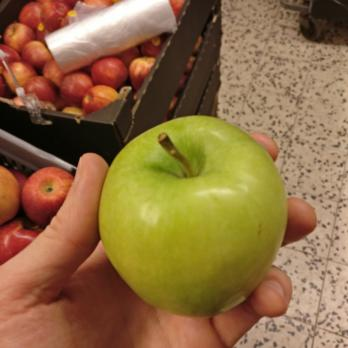
\includegraphics[height=1cm]{Chapter2/tikz/Golden-Delicious_031.jpg}};}},
}

\begin{tikzpicture}
	%\node at (0.5,-1){\begin{tabular}{c}input image\\layer $l = 0$\end{tabular}};
	\node at (0.5,2){\begin{tabular}{l}{\sf Inputs} \end{tabular}};
	\node at (2.,2){\begin{tabular}{l}{\sf Conv1} \end{tabular}};
	\node at (4.25,2){\begin{tabular}{l}{\sf Pooling1} \end{tabular}};
	\node at (6.2,2){\begin{tabular}{l}{\sf Conv2} \end{tabular}};
	\node at (8.8,2){\begin{tabular}{l}{\sf Pooling2} \end{tabular}};
	\node at (11.25,2){\begin{tabular}{l}{\sf FC} \end{tabular}};
	\node at (13.25,2){\begin{tabular}{l}{\sf Outputs} \end{tabular}};
	
	%\draw (0,0) -- (1,0) -- (1,1) -- (0,1) -- (0,0);
	\draw [path image,draw=black, thick] (0,0) rectangle (1,1);
	
	%\node at (3,3.5){\begin{tabular}{c}convolutional layer\\with non-linearities\\layer $l = 1$\end{tabular}};
	
	%\draw[fill=black,opacity=0.8,draw=black] (2.75,1.25) -- (3.75,1.25) -- (3.75,2.25) -- (2.75,2.25) -- (2.75,1.25);
	%\draw[fill=black,opacity=0.8,draw=black] (2.5,1) -- (3.5,1) -- (3.5,2) -- (2.5,2) -- (2.5,1);
	%\draw[fill=black,opacity=0.8,draw=black] (2.25,0.75) -- (3.25,0.75) -- (3.25,1.75) -- (2.25,1.75) -- (2.25,0.75);
	%\draw[fill=black,opacity=0.8,draw=black] (2,0.5) -- (3,0.5) -- (3,1.5) -- (2,1.5) -- (2,0.5);
	%\draw[fill=black,opacity=0.8,draw=black] (1.75,0.25) -- (2.75,0.25) -- (2.75,1.25) -- (1.75,1.25) -- (1.75,0.25);
	
	\draw[fill=black!50,opacity=0.8,draw=black] (2.0,0.5) -- (3.0,0.5) -- (3.0,1.5) -- (2.0,1.5) -- (2.0,0.5);
	\draw[fill=black!10,opacity=0.8,draw=black] (1.9,0.4) -- (2.9,0.4) -- (2.9,1.4) -- (1.9,1.4) -- (1.9,0.4);
	\draw[fill=black!50,opacity=0.8,draw=black] (1.8,0.3) -- (2.8,0.3) -- (2.8,1.3) -- (1.8,1.3) -- (1.8,0.3);
	\draw[fill=black!10,opacity=0.8,draw=black] (1.7,0.2) -- (2.7,0.2) -- (2.7,1.2) -- (1.7,1.2) -- (1.7,0.2);
	\draw[fill=black!50,opacity=0.8,draw=black] (1.6,0.1) -- (2.6,0.1) -- (2.6,1.1) -- (1.6,1.1) -- (1.6,0.1);
	\draw[fill=black!10,opacity=0.8,draw=black] (1.5,0) -- (2.5,0) -- (2.5,1) -- (1.5,1) -- (1.5,0);
	% conv box
	\draw (0.6,0.5) -- (0.8,0.5) -- (0.8,0.7) -- (0.6,0.7) -- (0.6,0.5);
	
	\draw (0.8,0.5) -- (2.2,0.6);
	\draw (0.8,0.7) -- (2.2,0.6);
	
	%\node at (4.5,-1){\begin{tabular}{c}subsampling layer\\layer $l = 3$\end{tabular}};
	
	%\draw[fill=black,opacity=0.8,draw=black] (5,1.25) -- (5.75,1.25) -- (5.75,2) -- (5,2) -- (5,1.25);
	%\draw[fill=black,opacity=0.8,draw=black] (4.75,1) -- (5.5,1) -- (5.5,1.75) -- (4.75,1.75) -- (4.75,1);
	%\draw[fill=black,opacity=0.8,draw=black] (4.5,0.75) -- (5.25,0.75) -- (5.25,1.5) -- (4.5,1.5) -- (4.5,0.75);
	%\draw[fill=black,opacity=0.8,draw=black] (4.25,0.5) -- (5,0.5) -- (5,1.25) -- (4.25,1.25) -- (4.25,0.5);
	%\draw[fill=black,opacity=0.8,draw=black] (4,0.25) -- (4.75,0.25) -- (4.75,1) -- (4,1) -- (4,0.25);
	%\draw[fill=black,opacity=0.8,draw=black] (3.75,0) -- (4.5,0) -- (4.5,0.75) -- (3.75,0.75) -- (3.75,0);
	
	\draw[fill=black!50,opacity=0.8,draw=black] (4.25,0.5) -- (5.0,0.5) -- (5.0,1.25) -- (4.25,1.25) -- (4.25,0.5);
	\draw[fill=black!10,opacity=0.8,draw=black] (4.15,0.4) -- (4.9,0.4) -- (4.9,1.15) -- (4.15,1.15) -- (4.15,0.4);
	\draw[fill=black!50,opacity=0.8,draw=black] (4.05,0.3) -- (4.8,0.3) -- (4.8,1.05) -- (4.05,1.05) -- (4.05,0.3);
	\draw[fill=black!10,opacity=0.8,draw=black] (3.95,0.2) -- (4.7,0.2) -- (4.7,0.95) -- (3.95,0.95) -- (3.95,0.2);
	\draw[fill=black!50,opacity=0.8,draw=black] (3.85,0.1) -- (4.6,0.1) -- (4.6,0.85) -- (3.85,0.85) -- (3.85,0.1);
	\draw[fill=black!10,opacity=0.8,draw=black] (3.75,0) -- (4.5,0) -- (4.5,0.75) -- (3.75,0.75) -- (3.75,0);
	
	% pooling box
	\draw (1.6,0.1) -- (1.8,0.1) -- (1.8,0.3) -- (1.6,0.3) -- (1.6,0.1);
	
	\draw (1.8,0.1) -- (3.9,0.15);
	\draw (1.8,0.3) -- (3.9,0.15);
	
	%\node at (7,3.5){\begin{tabular}{c}convolutional layer\\with non-linearities\\layer $l = 4$\end{tabular}};
	
	%\draw[fill=black,opacity=0.8,draw=black] (7.5,1.75) -- (8.25,1.75) -- (8.25,2.5) -- (7.5,2.5) -- (7.5,1.75);
	%\draw[fill=black,opacity=0.8,draw=black] (7.25,1.5) -- (8,1.5) -- (8,2.25) -- (7.25,2.25) -- (7.25,1.5);
	%\draw[fill=black,opacity=0.8,draw=black] (7,1.25) -- (7.75,1.25) -- (7.75,2) -- (7,2) -- (7,1.25);
	%\draw[fill=black,opacity=0.8,draw=black] (6.75,1) -- (7.5,1) -- (7.5,1.75) -- (6.75,1.75) -- (6.75,1);
	%\draw[fill=black,opacity=0.8,draw=black] (6.5,0.75) -- (7.25,0.75) -- (7.25,1.5) -- (6.5,1.5) -- (6.5,0.75);
	%\draw[fill=black,opacity=0.8,draw=black] (6.25,0.5) -- (7,0.5) -- (7,1.25) -- (6.25,1.25) -- (6.25,0.5);
	%\draw[fill=black,opacity=0.8,draw=black] (6,0.25) -- (6.75,0.25) -- (6.75,1) -- (6,1) -- (6,0.25);
	%\draw[fill=black,opacity=0.8,draw=black] (5.75,0) -- (6.5,0) -- (6.5,0.75) -- (5.75,0.75) -- (5.75,0);
	
	\draw[fill=black!50,opacity=0.8,draw=black] (6.65,0.9) -- (7.4,0.9) -- (7.4,1.65) -- (6.65,1.65) -- (6.65,0.9);			
	\draw[fill=black!10,opacity=0.8,draw=black] (6.55,0.8) -- (7.3,0.8) -- (7.3,1.55) -- (6.55,1.55) -- (6.55,0.8);			
	\draw[fill=black!50,opacity=0.8,draw=black] (6.45,0.7) -- (7.2,0.7) -- (7.2,1.45) -- (6.45,1.45) -- (6.45,0.7);	
	\draw[fill=black!10,opacity=0.8,draw=black] (6.35,0.6) -- (7.1,0.6) -- (7.1,1.35) -- (6.35,1.35) -- (6.35,0.6);		
	\draw[fill=black!50,opacity=0.8,draw=black] (6.25,0.5) -- (7.0,0.5) -- (7.0,1.25) -- (6.25,1.25) -- (6.25,0.5);
	\draw[fill=black!10,opacity=0.8,draw=black] (6.15,0.4) -- (6.9,0.4) -- (6.9,1.15) -- (6.15,1.15) -- (6.15,0.4);
	\draw[fill=black!50,opacity=0.8,draw=black] (6.05,0.3) -- (6.8,0.3) -- (6.8,1.05) -- (6.05,1.05) -- (6.05,0.3);
	\draw[fill=black!10,opacity=0.8,draw=black] (5.95,0.2) -- (6.7,0.2) -- (6.7,0.95) -- (5.95,0.95) -- (5.95,0.2);
	\draw[fill=black!50,opacity=0.8,draw=black] (5.85,0.1) -- (6.6,0.1) -- (6.6,0.85) -- (5.85,0.85) -- (5.85,0.1);
	\draw[fill=black!10,opacity=0.8,draw=black] (5.75,0) -- (6.5,0) -- (6.5,0.75) -- (5.75,0.75) -- (5.75,0);
	
	% conv box
	\draw (3.95,0.45) -- (4.15,0.45) -- (4.15,0.65) -- (3.95,0.65) -- (3.95,0.45);
	
	\draw (4.15,0.45) -- (6.05,0.55);
	\draw (4.15,0.65) -- (6.05,0.55);
	
	%\node at (9.5,-1){\begin{tabular}{c}subsampling layer\\layer $l = 6$\end{tabular}};
	
	%\draw[fill=black,opacity=0.8,draw=black] (10,1.75) -- (10.5,1.75) -- (10.5,2.25) -- (10,2.25) -- (10,1.75);
	%\draw[fill=black,opacity=0.8,draw=black] (9.75,1.5) -- (10.25,1.5) -- (10.25,2) -- (9.75,2) -- (9.75,1.5);
	%\draw[fill=black,opacity=0.8,draw=black] (9.5,1.25) -- (10,1.25) -- (10,1.75) -- (9.5,1.75) -- (9.5,1.25);
	%\draw[fill=black,opacity=0.8,draw=black] (9.25,1) -- (9.75,1) -- (9.75,1.5) -- (9.25,1.5) -- (9.25,1);
	%\draw[fill=black,opacity=0.8,draw=black] (9,0.75) -- (9.5,0.75) -- (9.5,1.25) -- (9,1.25) -- (9,0.75);
	%\draw[fill=black,opacity=0.8,draw=black] (8.75,0.5) -- (9.25,0.5) -- (9.25,1) -- (8.75,1) -- (8.75,0.5);
	%\draw[fill=black,opacity=0.8,draw=black] (8.5,0.25) -- (9,0.25) -- (9,0.75) -- (8.5,0.75) -- (8.5,0.25);
	%\draw[fill=black,opacity=0.8,draw=black] (8.25,0) -- (8.75,0) -- (8.75,0.5) -- (8.25,0.5) -- (8.25,0);
	\draw[fill=black!50,opacity=0.8,draw=black] (9.15,0.9) -- (9.65,0.9) -- (9.65,1.4) -- (9.15,1.4) -- (9.15,0.9);
	\draw[fill=black!10,opacity=0.8,draw=black] (9.05,0.8) -- (9.55,0.8) -- (9.55,1.3) -- (9.05,1.3) -- (9.05,0.8);
	\draw[fill=black!50,opacity=0.8,draw=black] (8.95,0.7) -- (9.45,0.7) -- (9.45,1.2) -- (8.95,1.2) -- (8.95,0.7);
	\draw[fill=black!10,opacity=0.8,draw=black] (8.85,0.6) -- (9.35,0.6) -- (9.35,1.1) -- (8.85,1.1) -- (8.85,0.6);
	\draw[fill=black!50,opacity=0.8,draw=black] (8.75,0.5) -- (9.25,0.5) -- (9.25,1.0) -- (8.75,1.0) -- (8.75,0.5);
	\draw[fill=black!10,opacity=0.8,draw=black] (8.65,0.4) -- (9.15,0.4) -- (9.15,0.9) -- (8.65,0.9) -- (8.65,0.4);
	\draw[fill=black!50,opacity=0.8,draw=black] (8.55,0.3) -- (9.05,0.3) -- (9.05,0.8) -- (8.55,0.8) -- (8.55,0.3);
	\draw[fill=black!10,opacity=0.8,draw=black] (8.45,0.2) -- (8.95,0.2) -- (8.95,0.7) -- (8.45,0.7) -- (8.45,0.2);
	\draw[fill=black!50,opacity=0.8,draw=black] (8.35,0.1) -- (8.85,0.1) -- (8.85,0.6) -- (8.35,0.6) -- (8.35,0.1);
	\draw[fill=black!10,opacity=0.8,draw=black] (8.25,0) -- (8.75,0) -- (8.75,0.5) -- (8.25,0.5) -- (8.25,0);
	
	% pooling box
	\draw (6.2,0.1) -- (6.4,0.1) -- (6.4,0.3) -- (6.2,0.3) -- (6.2,0.1);
	
	\draw(6.4,0.1) -- (8.65,0.15);
	\draw (6.4,0.3) -- (8.65,0.15);
	
	%\node at (12,3.5){\begin{tabular}{c}fully connected layer\\layer $l = 7$\end{tabular}};
	
	%\draw[fill=black,draw=black,opacity=0.5] (10.5,0) -- (11,0) -- (12.5,1.75) -- (12,1.75) -- (10.5,0);
	\draw[fill=black!10,draw=black,opacity=0.8] (10.5,0.1) -- (11,0.1) -- (11.8,1.0) -- (11.3,1.) -- (10.5,0.1);
	
	% flatten lines
	\draw(8.75,0.0) -- (10.5,0.1);
	\draw(9.65,1.4) -- (11.3,1.0);
	%\draw (6.4,0.3) -- (8.65,0.15);
	
	%\node at (13,-1){\begin{tabular}{c}fully connected layer\\output layer $l = 8$\end{tabular}};
	
	\draw[fill=black!10,draw=black,opacity=0.8] (12.5,0.0) -- (13,0.0) -- (13.45,0.6) -- (12.95,0.6) -- (12.5,0.0);
	
	% fc lines
	\draw(11.0,0.1) -- (12.5,0.0);
	\draw(11.8,1.0) -- (12.95,0.6);
\end{tikzpicture}